\chapterimage{images/mvvm/header.png}


\chapter{Architecture: from MVC to MVVM}

\section{Why}
A software project using a well-thought out architecture saves time: it allows for development of new features, it helps the programmer when existing features need to be changed, it is easy to test and provides the programmer with a sense of confidence, and so on. 
There are many different ways to architect an (Android) application: MVC, MVVM, MVI, MVP,\ldots 
Each have there own pros and cons, and it's up to the developer to know when the pick which.

The core idea of each architecture is the same however: separation of concerns.
The responsibilities of each class or module should be clearly defined and all these component should work together in a well-structured way. 
How this is done is different for each architecture. 

Some architectures are better supported by the (Android) framework than others. 
``Base'' Android is mostly MVC (Model, View, Controller), but with the release of the Android Architecture Components came more support for a MVVM (Model, View, ViewModel) approach.
The next two sections cover both, but in this course we will study MVVM more in depth. 


%Base Android: Controller is Activity/Fragment, Model is the Model, View is Layout
%Probleem is dat Controller in Android zo gelinkt is aan architectuur dat die niet getest kan worden.
%Moet ook veel doen: model bijhouden, updaten, UI listenen,...
%Later zal VM de repo bijhouden, activity wordt steeds kleiner

\section{MVC}
MVC is one of the more common architectural software patterns.
It divides your code into three interconnected parts \cite{mvc-mvp-mvv-on-android}:

\begin{description}
	\item[Model:] the central data and state of the application, together with the business logic.
	\item[View:] the representation of the model. Its responsibility is to render the UI.
	\item[Controller:] acts as an agent between the model and the view. 
		When the view receives user input, the controller will interact with the model to attain the desired effects.
\end{description}

Figure \ref{fig:MVCdiagram} illustrates the role of standard Android Components such as layout files, \lstinline!Activities! and \lstinline!Fragments! in MVC.
Normally MVC is a good way to architect your application, but in Android specifically there are some issues:

\begin{enumerate}
	\item Unit Testing the \lstinline!Activities! and \lstinline!Fragments! is extremely difficult because they are so tied in to the Android Framework.
	``God'' objects such as Context and the \lstinline!Activity! life cycle all stand in the way of easy testing.
	\item \lstinline!Activities! and \lstinline!Fragments! as controllers have many responsibilities. 
	They have to keep the UI (View) up-to-date, interact with databases or remote API's, correctly implement the life cycle,\ldots
	This makes for lots of code which becomes harder to maintain over time.
	\item Controllers and Views are tightly coupled: changing something in a layout file is very likely to mean changes in the controller as well. 
\end{enumerate}

\begin{figure}[ht]
	\centering
	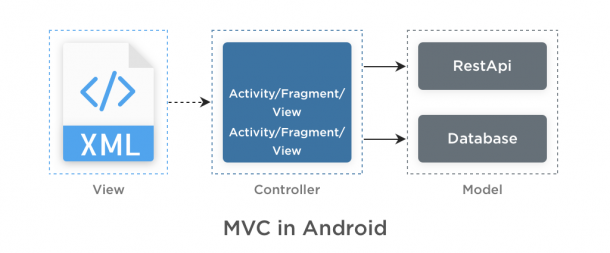
\includegraphics[width=\textwidth]{images/mvvm/MVC_diagram.png}
	\label{fig:MVCdiagram}
	\caption{A diagram illustrating the MVC architecture in Android. From \cite{simform}.}
\end{figure}

Luckily, there are a better way to organize your code: through architectural patterns such as MVVM, MVI, MVP,\ldots

All have gained some popularity in the Android community, but the recently released architecture components \cite{architectureComponents} focus quite heavily on MVVM.
In this course we will make much use of these components and as such use MVVM as our architecture of choice.

\section{MVVM}
In this section we explore the MVVM architecture step-by-step. 
We start by looking at the concept of a \lstinline!ViewModel! class, and how it helps us with the issue of configuration changes.
After that has been made clear, we use this \lstinline!ViewModel! class to be part of an MVVM architecture. 
Lastly we look at another use case for the \lstinline!ViewModel! class: a way to allow \todo{continue sentence}

\subsection{ViewModel as a way to survive configuration changes}
We have discussed the problem of saving and restoring state already in section \ref{sec:saveAndRestoreState}. 
There the \lstinline!onSaveInstanceState! and \lstinline!onCreate! methods were proposed as a solution.
A short example of this can be seen in listing \ref{code:basicMVC}.

\lstinputlisting[language=Kotlin, 
caption={A simple application with a \lstinline!TextView!, an \lstinline!EditText! and a \lstinline!Button!.
	After pressing the button, the text in the \lstinline!TextView! is updated with the user's input in the \lstinline!EditText!.
	Saving and Restoring UI state is done using the \lstinline!onSaveInstanceState! method.},
label=code:basicMVC]{srccode/mvvm/MVC_simple/app/src/main/java/be/hogent/nativeapps/mvc_example/MainActivity.kt}

However, there is another solution: using a \lstinline!ViewModel! class.
This class is part of the Android Lifecycle Architecture Components \cite{viewModelOfficial}.
While the concept of a viewmodel isn't specific to Android, this implementation is of particular interest to us because it ties in to the \lstinline!Activity! lifecycle.

The \lstinline!ViewModel! class is part of the Android Lifecycle Extensions Library.
To use this library it has to be added as a dependency of your application.
This means the following line has to be added to your app module's gradle file:

\begin{android}
	implementation "android.arch.lifecycle:extensions:1.1.1"
\end{android}


A generic viewmodel class is used as part of an MVVM architecture (more on that later), and its job is to hold all elements of the model that are exposed in the UI.

This reduces the size and complexity of what would normally be the controller.
In our case, it is exactly those pieces of data that we normally lose during configuration changes.
We could make that generic viewmodel class \lstinline!Serializable! and use \lstinline!onSaveInstanceState! and \lstinline!onCreate! to save and restore it, but there is an easier way. 

The ViewModel class that is a part of the Android Architecture Components isn't one that you create yourself using a regular constructor, but by using a \lstinline!ViewModelProvider! \cite{viewModelProvider}.
In the \lstinline!onCreate! function of your \lstinline!Fragment! or \lstinline!Activity! you use the following line of code to instantiate your \lstinline!ViewModel!.


\begin{android}
val model = ViewModelProviders.of(this).get(MyViewModel::class.java)	
\end{android}

The \lstinline!this! refers to the \lstinline!Activity! itself, and links the \lstinline!ViewModel! to the \lstinline!Activity's! lifecycle.

\lstinline!ViewModelProviders! keeps a list of all active life cycles and the associated \lstinline!ViewModels!.
\footnote{This becomes especially important when using \lstinline!ViewModels! for sharing data between \lstinline!Fragments!.
Using the example of a dual-pane layout: both the \lstinline!ListFragment! and \lstinline!DetailFragment! would need to specify the \lstinline!Activity! that hosts them both when creating the \lstinline!ViewModel! in order to both receive the same instance. 
More information on this can be found in \cite{shareDataBetweenFragments}.}

When a configuration change occurs, the \lstinline!ViewModelProvider! still has a reference to the created \lstinline!ViewModel! and can just return it.
This alleviates the need for \lstinline!onSaveInstanceState! for configuration change state changes. 

An example implementation can be seen in \ref{code:viewModelActivity} (the \lstinline!Activity! class) and \ref{code:viewModelSimple} (the \lstinline!ViewModel! class).
In more realistic applications the \lstinline!ViewModel! would hold much more than just one piece of UI information.

Every part of the UI that gets data from the model should be retained in the \lstinline!ViewModel!.

\lstinputlisting[language=Kotlin,
caption={A very simple application with a \lstinline!TextView!, an \lstinline!EditText! and a \lstinline!Button!.
	After pressing the button, the text in the \lstinline!TextView! is updated with the user's input in the \lstinline!EditText!.
	Saving and Restoring UI state is done using a \lstinline!ViewModel!.},
label=code:viewModelActivity]{srccode/mvvm/ViewModel_simple/app/src/main/java/be/hogent/nativeapps/mvc_example/MainActivity.kt}

\lstinputlisting[language=Kotlin,
caption={The InputViewModel class that is used in listing \ref{code:viewModelActivity}.
	It extends the abstract ViewModel class from the Android Architecture Components.},
label=code:viewModelSimple]{srccode/mvvm/ViewModel_simple/app/src/main/java/be/hogent/nativeapps/mvc_example/InputViewModel.kt}

\subsection{ViewModel with Data Binding and LiveData as part of an MVVM architecture}

Extracting the UI state from the \lstinline!Activity! as done in the previous section is the first step towards a full MVVM architecture.
MVVM is composed of 3 parts, as illustrated in \ref{fig:MVVMdiagram}
\begin{description}
	\item[Model:] the central data and state of the application, together with the business logic.
	\item[View:] the representation of the model. Its responsibility is to render the UI.
				In contrast with MVC, in MVVM the  \lstinline!Activity! or  \lstinline!Fragment! is also considered part of the View.
	\item[ViewModel:] a container that wraps (part of) the model and provides observable data needed by the view.
	It also provides hooks for the view to pass events to the model. The ViewModel is not tied to the view however.
\end{description}

\begin{figure}[ht]
	\centering
	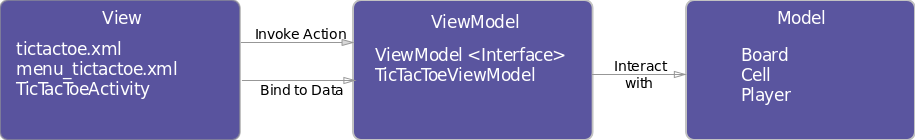
\includegraphics[width=\textwidth]{images/mvvm/MVVM.png}
	\label{fig:MVVMdiagram}
	\caption{A diagram illustrating the MVVM architecture in Android.
		Here it is applied to a Tic-Tac-Toe game.
		From \cite{mvc-mvp-mvv-on-android}.}
\end{figure}

The responsibilities and direction of communication are a bit different from what we are used to.
The \lstinline!Activity! or \lstinline!Fragment! will no longer configure each piece of the UI, instead the UI gets its data from a \lstinline!ViewModel! directly.
Actions aren't registered in the \lstinline!Activity!, but are sent from layout to the \lstinline!ViewModel!, which in turn communicates with the model.
Communication with the Android Framework in order to switch screens will have to be done in a way that requires complete separation between the ViewModel and the \lstinline!Activity! or \lstinline!Fragment!.
Each of these three requirements are discussed in a separate section.

\subsubsection{Binding the ViewModel to the View}
If we want the View to bind to data from the \lstinline!ViewModel! 
This is done using the Data Binding library \cite{dataBinding}.
It allows you to add a link to a \lstinline!ViewModel! (or other model classes) directly into your layout files.

Any UI component that needs a piece of data from the \lstinline!ViewMode!l can request it directly from the \lstinline!ViewModel!.
This reduces the role of the \lstinline!Activity! even more: it is no longer responsible for updating the \lstinline!View!.

The first step is transforming the normal layout into one that supports data binding.
This involves creating a variable in the layout file that will hold a reference to the ViewModel.
Listing \ref{code:dataBindingXMLvariable} illustrates this step.

\lstinputlisting[language=XML, firstline=2,lastline=8,
caption={The entire layout is wrapped by a <layout> tag, and a variable is defined to hold the ViewModel},
label=code:dataBindingXMLvariable]{srccode/mvvm/ViewModel_DataBinding_LiveData/app/src/main/res/layout/activity_main.xml}

UI components can then reference this variable when they require a piece of UI state, as shown in listing \ref{code:dataBindingXMLreference}.

\lstinputlisting[language=XML, firstline=16,lastline=21,
caption={XML attributes can reference the variable to fill their values.},
label=code:dataBindingXMLreference]{srccode/mvvm/ViewModel_DataBinding_LiveData/app/src/main/res/layout/activity_main.xml}

\subsubsection{Automatically updating the UI on state changes}
The matter of updating state of the UI when a user interacts with it can be solved using the LiveData Architecture Component \cite{liveData}.

A LiveData object is an observable object. This means that other objects can first register and subsequently listen to changes in the value of that object.
This functionality alone could also be provided using Observable objects\cite{observable}.
LiveData however has much more to offer: it is completely linked with the listener's lifecycle. This means no problems during configuration changes, no memory leaks, no updates send to inactive (and possibly destroyed) listeners resulting in crashes \ldots

Using LiveData means making minor changes to both the \lstinline!ViewModel! and the \lstinline!Activity!, as seen in listing \ref{code:dataBindingViewModel}

In the \lstinline!ViewModel! the attributes are now wrapped inside \lstinline!LiveData! objects.
This provides all lifecycle and observable functionality. 

\lstinputlisting[language=Kotlin,
caption={Attributes in the \lstinline!ViewModel! are wrapped inside \lstinline!LiveData! objects. Sometimes some extra initialization code is needed.},
label=code:dataBindingViewModel]{srccode/mvvm/ViewModel_DataBinding_LiveData/app/src/main/java/be/hogent/nativeapps/mvc_example/InputViewModel.kt}

In the \lstinline!Activity! there are 3 things to do:
\begin{inparaenum}[(i)]
	\item ask for the binding with the layout file,
	\item binding the \lstinline!ViewModel! to the layout and
	\item setting the \lstinline!LifeCycleOwner!.
\end{inparaenum}

We need the binding to link fill in the variables defined in the layout file. 
Setting the \lstinline!LifeCycleOwner! is needed when using \lstinline!LiveData!. 
Without this step the LiveData objects can't know when their listeners are active or not. All three steps are illustrated in listing \ref{code:dataBindingActivity}.


\lstinputlisting[language=Kotlin,firstline=14, lastline=31,
caption={Attributes in the \lstinline!ViewModel! are wrapped inside \lstinline!LiveData! objects. Sometimes some extra initialization code is needed.},
label=code:dataBindingActivity]{srccode/mvvm/ViewModel_DataBinding_LiveData/app/src/main/java/be/hogent/nativeapps/mvc_example/MainActivity.kt}

\subsubsection{Responding to events that require Activity or Fragment}
A very important espect of the \lstinline!ViewModel! is that it should \textbf{never} hold any references to a \lstinline!View!, be it a \lstinline!Activity! or a \lstinline!Fragment!.
This is because \lstinline!ViewModels! are designed to survive configuration changes, and \lstinline!Views! are not.
So holding a reference to a \lstinline!View! that has been destroyed will lead to crashes. 

This leads to the problem of how to responds to user interactions that require, for example, a new screen to be shown.
To start a new \lstinline!Activity! or \lstinline!Fragment! you need to have a reference to one.
But we can't, because a \lstinline!ViewModel! can't hold these references!

To solve this, we allow \lstinline!Activities! and \lstinline!Fragments! to observe special events produced by their \lstinline!ViewModels!.
Using the same \lstinline!LiveData! library from before we can make a special kind of observable object 
(an instance of \lstinline!SingeLiveEvent!\footnote{\url{https://raw.githubusercontent.com/hdeweirdt/CriminalIntent/viewmodel/app/src/main/java/com/deweirdt/harm/criminalIntent/util/SingleLiveEvent.kt}}) 
that we will cause to update whenever the user indicates they want to go to another screen.
The \lstinline!Activity! or \lstinline!Fragment! will observe this object and react to the event by following the usual steps to start a new \lstinline!Activity! or \lstinline!Fragment!.

The \lstinline!ViewModel! code is illustrated in figure \ref{code:ViewModelEvent}.
The \lstinline!Fragment! code is illustrated in figure \ref{code:FragmentEvent}.
	
\begin{lstlisting}[language=Kotlin, label=code:ViewModelEvent,
caption={The \lstinline!ViewModel! has one \lstinline!SingeLiveEvent! for each interaction that eventually requires action from a \lstinline!Activity! or \lstinline!Fragment!.
The \lstinline!onButtonClicked! functions are referenced in the layout files.}]
val suspectButtonEvent = SingleLiveEvent<Unit>()

fun onSuspectButtonClicked(button: View) {
	suspectButtonEvent.call()
}
\end{lstlisting}

\begin{lstlisting}[language=Kotlin,label=code:FragmentEvent,
caption={The \lstinline!Activities! or \lstinline!Fragments! observe the events from the  \lstinline!ViewModel!, and respond by creating a new \lstinline!Activity! or \lstinline!Fragment!}]
 override fun onStart() {
	super.onStart()
	mCrimeViewModel.suspectButtonEvent.observe(this, Observer { suspectButtonClicked() })
}
private fun suspectButtonClicked() {
	val pickContact = Intent(Intent.ACTION_PICK, ContactsContract.Contacts.CONTENT_URI)
	startActivityForResult(pickContact, REQUEST_CONTACT)
}
\end{lstlisting}